\begin{center}
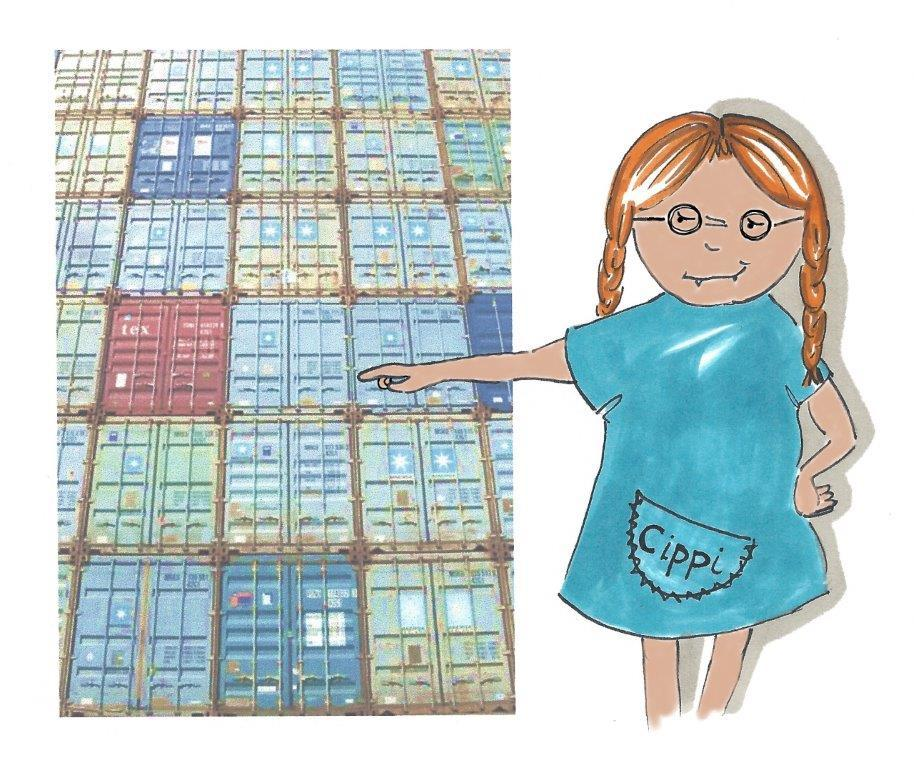
\includegraphics[width=0.6\textwidth]{content/3/chapter5/images/10.png}\\
Cippi在检查集装箱
\end{center}

C++20对标准模板库的容器还进行了很多改进。首先,std::vector和std::string添加了constexpr构造函数,从而可以在编译时使用。所有容器都支持统一的erase成员函数,以及关联容器(map/set)添加了成员函数contains。此外,std::string可以对前缀或后缀进行检查。

\subsubsubsection{5.3.1\hspace{0.2cm}constexpr的容器和算法}

C++20支持constexpr容器std::vector和std::string,其中constexpr表明这两个容器的成员函数都可以在编译时使用。此外,标准模板库中,声明为constexpr的\href{https://en.cppreference.com/w/cpp/algorithm}{算法}超过了100个。

因此,可以在编译时对int类型的std::vector进行排序。

\begin{lstlisting}[style=styleCXX]
// constexprVector.cpp

#include <algorithm>
#include <iostream>
#include <vector>

constexpr int maxElement() {
	std::vector myVec = {1, 2, 4, 3};
	std::sort(myVec.begin(), myVec.end());
	return myVec.back();
}
int main() {

	std::cout << '\n';
	
	constexpr int maxValue = maxElement();
	std::cout << "maxValue: " << maxValue << '\n';
	
	constexpr int maxValue2 = [] {
		std::vector myVec = {1, 2, 4, 3};
		std::sort(myVec.begin(), myVec.end()) ;
		return myVec.back();
	}();
	
	std::cout << "maxValue2: " << maxValue2 << '\n';
	
	std::cout << '\n';

}
\end{lstlisting}

两个std::vector(第8行和第20行)在编译时使用constexpr声明的函数进行排序。第一种情况下,函数maxElement返回myVec的最后一个元素,也就是它的最大值。第二种情况下,使用声明为constexpr的Lambda表达式。

\begin{tcblisting}{commandshell={}}
maxValue: 4
maxValue2: 4
\end{tcblisting}

\subsubsubsection{5.3.2\hspace{0.2cm}std::array}

C++20提供了两种创建数组的方法。std::to\_array可以创建std::array,而std::make\_shared现在可以创建std::shared\_ptr数组了。

\hspace*{\fill} \\ %插入空行
\noindent
\textbf{5.3.2.1\hspace{0.2cm}std::to\_array}

std::to\_array从现有一维数组创建std::array,其中的元素是从现有的一维数组复制过来的。

一维数组可以是C-string、std::initializer\_list或std::pair的一维数组。下面的例子来自\href{https://en.cppreference.com/w/cpp/container/array/to_array}{cppreference.com/to\_array}。

\begin{lstlisting}[style=styleCXX]
// toArray.cpp

#include <iostream>
#include <utility>
#include <array>
#include <memory>

int main() {

	std::cout << '\n';
	
	auto arr1 = std::to_array("A simple test");
	for (auto a: arr1) std::cout << a;
	std::cout << "\n\n";
	
	auto arr2 = std::to_array({1, 2, 3, 4, 5});
	for (auto a: arr2) std::cout << a;
	std::cout << "\n\n";
	
	auto arr3 = std::to_array<double>({0, 1, 3});
	for (auto a: arr3) std::cout << a;
	std::cout << '\n';
	std::cout << "typeid(arr3[0]).name(): " << typeid(arr3[0]).name() << '\n';
	std::cout << '\n';
	
	auto arr4 = std::to_array<std::pair<int, double>>({ {1, 0.0}, {2, 5.1},
	{3, 5.1} });
	for (auto p: arr4) {
		std::cout << "(" << p.first << ", " << p.second << ")" << '\n';
	}
	
	std::cout << "\n\n";

}
\end{lstlisting}

使用C-string(第12行),std::initializer\_list(第16行和第20行),std::pair的std::initializer\_list(第26行)都可以创建std::array。通常,编译器可以推断出std::array的类型,还可以对类型进行指定(第20和26行)。

\begin{tcblisting}{commandshell={}}
A simple test

12345

013

typeid(arr3[0]).name(): d

(1, 0)
(2, 5.1)
(3, 5.1)
\end{tcblisting}

\hspace*{\fill} \\ %插入空行
\noindent
\textbf{5.3.2.2\hspace{0.2cm}std::make\_shared}

C++11的工厂函数\href{https://en.cppreference.com/w/cpp/memory/shared_ptr/make_shared}{std::make\_shared}用于创建std::shared\_ptr。C++20中,这个工厂函数终于支持创建std::shared\_ptr数组了。

\begin{itemize}
\item 
std::shared\_ptr<double[]> sha = std::make\_shared<double[]>(1024):创建一个shared\_ptr,默认初始化1024个double变量

\item 
std::shared\_ptr<double[]> shar = std::make\_shared<double[]>(1024, 1.0): 创建了一个shared\_ptr,其中1024个double初始化为1.0
\end{itemize}

\subsubsubsection{5.3.3\hspace{0.2cm}擦除功能}

C++20之前,从容器中删除元素太麻烦了。

\hspace*{\fill} \\ %插入空行
\noindent
\textbf{5.3.3.1\hspace{0.2cm}erase-remove习语}

从容器中删除元素好像很容易。对于std::vector,可以使用std::remove\_if函数。

\begin{lstlisting}[style=styleCXX]
// removeElements.cpp

#include <algorithm>
#include <iostream>
#include <vector>

int main() {

	std::cout << '\n';
	
	std::vector myVec{-2, 3, -5, 10, 3, 0, -5 };
	
	for (auto ele: myVec) std::cout << ele << " ";
	std::cout << "\n\n";
	
	std::remove_if(myVec.begin(), myVec.end(), [](int ele){ return ele < 0; });
	for (auto ele: myVec) std::cout << ele << " ";
	
	std::cout << "\n\n";

}
\end{lstlisting}

removeElements.cpp从std::vector中删除所有小于零的元素。很容易,对吧?或许也并不容易;现在,您可能陷入了资深C++程序员所熟知的陷阱。

\begin{center}
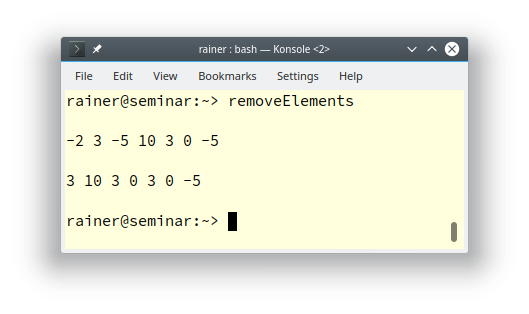
\includegraphics[width=0.7\textwidth]{content/3/chapter5/images/11.png}\\
\end{center}

std::remove\_if(第16行)不会删除任何东西,std::vector的元素数量不变。算法只是返回修改后容器的新(逻辑)末端。

为了修改容器内容,必须将新末端应用于容器。

\begin{lstlisting}[style=styleCXX]
// eraseRemoveElements.cpp

#include <algorithm>
#include <iostream>
#include <vector>

int main() {
	
	std::cout << '\n';
	
	std::vector myVec{-2, 3, -5, 10, 3, 0, -5 };
	
	for (auto ele: myVec) std::cout << ele << " ";
	std::cout << "\n\n";
	
	auto newEnd = std::remove_if(myVec.begin(), myVec.end(),
	[](int ele){ return ele < 0; });
	myVec.erase(newEnd, myVec.end());
	// myVec.erase(std::remove_if(myVec.begin(), myVec.end(),
	//              [](int ele){ return ele < 0; }), myVec.end());
	for (auto ele: myVec) std::cout << ele << " ";
	
	std::cout << "\n\n";

}
\end{lstlisting}

第16行返回容器myVec的新末端newEnd。这个新末端应用于第18行,并从newEnd开始删除myVec中的元素。当在表达式中应用函数remove和erase(第19行)时,就会清楚地了解为什么这种方式称为“erase-remove习语”了。

\begin{center}
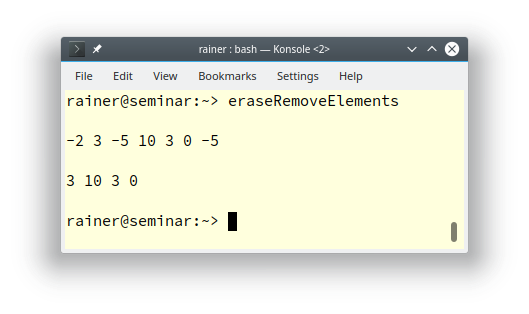
\includegraphics[width=0.7\textwidth]{content/3/chapter5/images/12.png}\\
\end{center}

因为C++20中新增了erase和erase\_if,从容器中擦除元素就方便了许多。

\hspace*{\fill} \\ %插入空行
\noindent
\textbf{5.3.3.2\hspace{0.2cm}C++20的erase和erase\_if}

使用erase和erase\_if,可以直接对容器进行操作。相比之下,前面介绍的erase-remove习语看上去就相当麻烦了:迭代了两次。

来一起看看新函数erase和erase\_if在实践中怎么使用。下面的代码,是从容器中删除一些元素。

\begin{lstlisting}[style=styleCXX]
// eraseCpp20.cpp

#include <iostream>
#include <numeric>
#include <deque>
#include <list>
#include <string>
#include <vector>

template <typename Cont>
void eraseVal(Cont& cont, int val) {
	std::erase(cont, val);
}

template <typename Cont, typename Pred>
void erasePredicate(Cont& cont, Pred pred) {
	std::erase_if(cont, pred);
}

template <typename Cont>
void printContainer(Cont& cont) {
	for (auto c: cont) std::cout << c << " ";
	std::cout << '\n';
}

template <typename Cont>
void doAll(Cont& cont) {
	printContainer(cont);
	eraseVal(cont, 5);
	printContainer(cont);
	erasePredicate(cont, [](auto i) { return i >= 3; } );
	printContainer(cont);
}

int main() {

	std::cout << '\n';
	
	std::string str{"A Sentence with an E."};
	std::cout << "str: " << str << '\n';
	std::erase(str, 'e');
	std::cout << "str: " << str << '\n';
	std::erase_if( str, [](char c){ return std::isupper(c); });
	std::cout << "str: " << str << '\n';
	
	std::cout << "\nstd::vector " << '\n';
	std::vector vec{1, 2, 3, 4, 5, 6, 7, 8, 9};
	doAll(vec);
	
	std::cout << "\nstd::deque " << '\n';
	std::deque deq{1, 2, 3, 4, 5, 6, 7, 8, 9};
	doAll(deq);
	
	std::cout << "\nstd::list" << '\n';
	std::list lst{1, 2, 3, 4, 5, 6, 7, 8, 9};
	doAll(lst);

}
\end{lstlisting}

第41行删除给定字符串str中的所有'e'字符。第43行将Lambda表达式应用于同一字符串,并删除了所有大写字母。

代码的其余部分,删除了std::vector(第47行)、std::deque(第51行)和std::list(第55行)的相应元素。对每个容器上应用函数模板doAll(第26行),doAll删除元素5和所有大于或等于3的元素。函数模板eraseVal(第10行)使用新的erase函数,函数模板erasePredicate(第15行)使用新的函数erase\_if。

\begin{center}
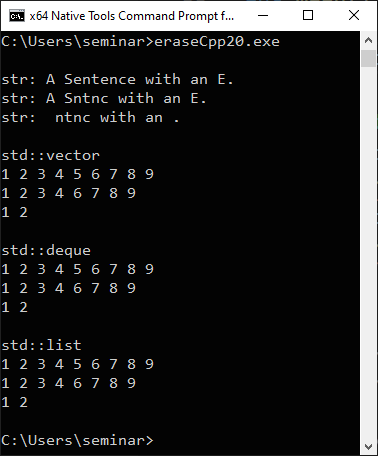
\includegraphics[width=0.5\textwidth]{content/3/chapter5/images/13.png}\\
\end{center}

新函数erase和erase\_if可以应用于标准模板库的所有容器。但这并不适用于另一个函数contains,其需要对关联容器进行操作。

\subsubsubsection{5.3.4\hspace{0.2cm}关联容器的contains}

由于contains函数,就可以轻松地检查关联容器中是否存在元素。你可能会说,我们已经可以用find或count来完成这个任务了。

非也非也,这两个函数都不适合初学者,而且有各自的缺点。

\begin{lstlisting}[style=styleCXX]
// checkExistence.cpp

#include <set>
#include <iostream>

int main() {

	std::cout << '\n';
	
	std::set mySet{3, 2, 1};
	if (mySet.find(2) != mySet.end()) {
		std::cout << "2 inside" << '\n';
	}
	
	std::multiset myMultiSet{3, 2, 1, 2};
	if (myMultiSet.count(2)) {
		std::cout << "2 inside" << '\n';
	}
	
	std::cout << '\n';

}
\end{lstlisting}

函数产生预期的结果。

\begin{tcblisting}{commandshell={}}
2 inside
2 inside
\end{tcblisting}

\begin{center}
使用find和count检查容器中是否有给定的元素
\end{center}

两个方式都有问题。find(第11行)太冗长了,count(第16行)也是,count还存在性能上的问题。想知道某个元素是否在容器中时,应该在找到时停止,而不是继续查找直到结束。上面的代码中,myMultiSet.count(2)会返回2。

与find和count不同,C++20中的contains成员函数使用起来非常方便。

\begin{lstlisting}[style=styleCXX]
// containsElement.cpp

#include <iostream>
#include <set>
#include <map>
#include <unordered_set>
#include <unordered_map>

template <typename AssocCont>
bool containsElement5(const AssocCont& assocCont) {
	return assocCont.contains(5);
}

int main() {

	std::cout << std::boolalpha;
	
	std::cout << '\n';
	
	std::set<int> mySet{1, 2, 3, 4, 5, 6, 7, 8, 9, 10};
	std::cout << "containsElement5(mySet): " << containsElement5(mySet);
	
	std::cout << '\n';
	
	std::unordered_set<int> myUnordSet{1, 2, 3, 4, 5, 6, 7, 8, 9, 10};
	std::cout << "containsElement5(myUnordSet): " << containsElement5(myUnordSet);
	
	std::cout << '\n';
	
	std::map<int, std::string> myMap{ {1, "red"}, {2, "blue"}, {3, "green"} };
	std::cout << "containsElement5(myMap): " << containsElement5(myMap);
	
	std::cout << '\n';
	
	std::unordered_map<int, std::string> myUnordMap{ {1, "red"},
	                                                 {2, "blue"}, {3, "green"} };
	std::cout << "containsElement5(myUnordMap): " << containsElement5(myUnordMap);
	
	std::cout << '\n';

}
\end{lstlisting}

若关联容器包含键5,则函数模板containsElement5返回true。例子中,我只使用了关联容器std::set、std::unordered\_set、std::map和std::unordered\_set,它们都不能多次保存给定的键。

\begin{center}
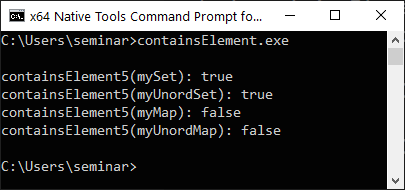
\includegraphics[width=0.6\textwidth]{content/3/chapter5/images/14.png}\\
\end{center}

\subsubsubsection{5.3.5\hspace{0.2cm}字符串检查前缀和后缀}

std::string获取新的成员函数starts\_with和ends\_with,可以检查std::string是否以指定的子字符串开始或结束。

\begin{lstlisting}[style=styleCXX]
// stringStartsWithEndsWith.cpp

#include <iostream>
#include <string_view>
#include <string>

template <typename PrefixType>
void startsWith(const std::string& str, PrefixType prefix) {
	std::cout << " starts with " << prefix << ": "
			  << str.starts_with(prefix) << '\n';
}

template <typename SuffixType>
void endsWith(const std::string& str, SuffixType suffix) {
	std::cout << " ends with " << suffix << ": "
			  << str.ends_with(suffix) << '\n';
}

int main() {

	std::cout << '\n';
	
	std::cout << std::boolalpha;
	
	std::string helloWorld("Hello World");
	
	std::cout << helloWorld << '\n';
	
	startsWith(helloWorld, helloWorld);
	
	startsWith(helloWorld, std::string_view("Hello"));
	
	startsWith(helloWorld, 'H');
	
	std::cout << "\n\n";
	
	std::cout << helloWorld << '\n';
	
	endsWith(helloWorld, helloWorld);
	
	endsWith(helloWorld, std::string_view("World"));
	
	endsWith(helloWorld, 'd');

}
\end{lstlisting}

starts\_with和ends\_with的成员函数都是谓词,返回布尔值。可以用std::string(第29行和39行),std::string\_view(第31行和41行)和char(第33行和43行)使用新的成员函数。

\begin{tcblisting}{commandshell={}}
Hello World
            starts with Hello World: true
            starts with Hello: true
            starts with H: true
            
Hello World
            ends with Hello World: true
            ends with World: true
            ends with d: true
\end{tcblisting}

\begin{tcolorbox}[breakable,enhanced jigsaw,colback=mygreen!5!white,colframe=mygreen!75!black,title={总结}]
	
\begin{itemize}
\item 
std::vector和std::string具有constexpr构造函数,可以在编译时实例化。由于标准模板库(STL)提供constexpr算法,可以在编译时执行。

\item 
C++20提供了两种创建数组的方法。std::to\_array创建std::array,std::make\_shared可以创建包含数组的std::shared\_ptr。

\item 
新的算法std::erase和std::erase\_if用于从STL容器中删除特定的元素(erase)或满足谓词(erase\_if)的元素。

\item 
有了新成员函数contains,就可以直接检查关联容器是否具有所请求的键。

\item 
std::string支持新的成员函数start\_with和end\_with,可用来检查容器是否具有特定的前缀或后缀。
\end{itemize}
	
\end{tcolorbox}


\newpage


















